\section{Realisierung}
\subsection{Vorgehensweise}
Zu Beginn wurde ein Plan für das grobe Zusammenspiel der beteiligten
Komponenten angefertigt. Hiermit wurde die Arbeit in mehrere Schritte
und leicht abzugrenzende Komponenten unterteilt. Das Projekt ließ sich
damit in Meilensteine aufteilen, um strukturiert an das Projekt
herangehen zu können. Als Vorgehensweise wurde das erweiterte
Wasserfall-Modell gewählt\ref{fig:wasserfall_modell}.
\begin{figure}[h]
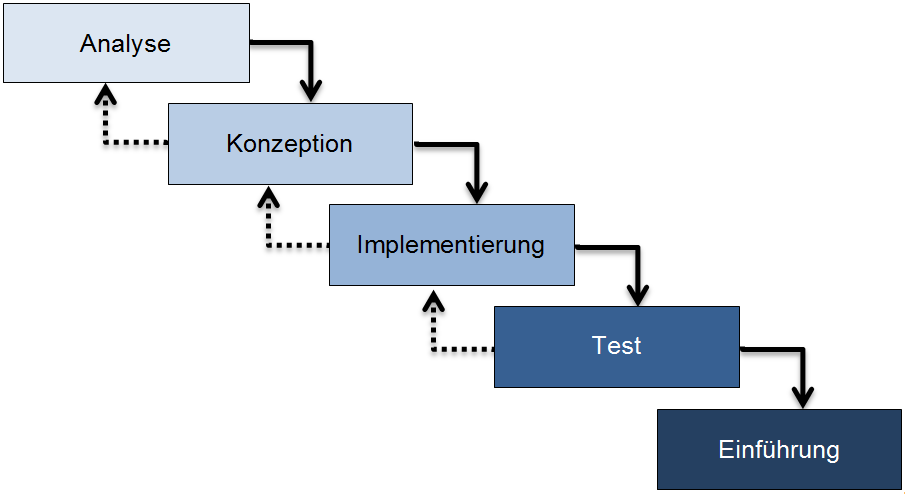
\includegraphics[scale=0.5]{img/wasserfall_modell.png}
\caption{Erweitertes Wasserfallmodell\label{fig:wasserfall_modell}}
\end{figure}
Aufgrund der knappen Zeitanforderungen bietet ein solcher Ansatz
einen direkten, klaren Pfad vom Beginn zum Ende des Projektes. Im
erweiterten Wasserfall-Modell erhält man, durch die Möglichkeit
Rückschritte zu machen, die nötige Flexibilität um auf Feedback
einzugehen und Dinge ausprobieren zu können.
\subsection{Analyse \& Konzeption}
Bei der Analyse der Anforderungen fallen die Realtime Aspekte auf. Sie
sollen mithilfe von Websocketkommunikation und Push-Based-Updates vom
Server umgesetzt werden. Für einen modernen Look und ein intuitives
Verhalten auf mobilen Geräten soll die Steuerung Drag and Drop unterstützen.
\subsubsection{Architektur}
Einen groben Überblick über die spätere ``physikalische Ausprägung''
des Systems soll Abbildung~\ref{fig:architektur} geben.
\begin{figure}[h]
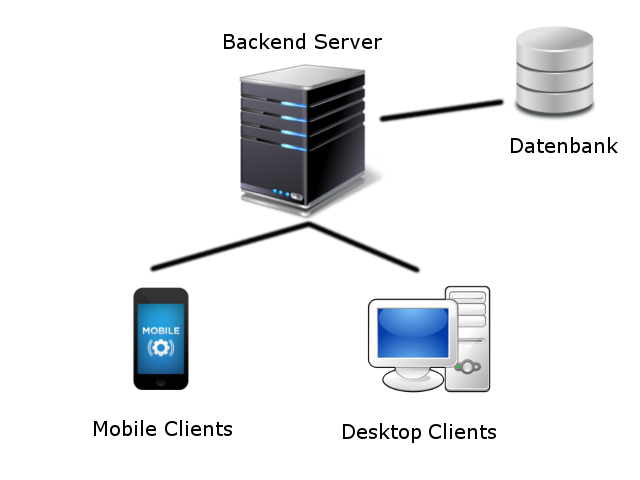
\includegraphics[scale=0.5]{img/Architektur.png}
\caption{Architektur Übersicht\label{fig:architektur}}
\end{figure}
Die Clients (Mobile / Desktop) kommunizieren über WebSockets mit dem
Backend-Server. Dieser speichert und liest Daten aus einer Datenbank.
Durch die WebSockets ist es dem Backend-Server möglich Änderungen am
Datenmodell mittels Push-Benachrichtigungen an die Clients weiterzugeben.
\subsection{Implementierung}
\subsubsection{Browser-Frontend}
Die Implementierung des Browser-Frontends verwendet Technologien, die
dem Reactive Pattern zuzuweisen sind. React.js als UI-Framework von
Facebook ist ein stark durch funktionale Ideen inspiriertes Framework.
Das Browser Frontend ist modular aufgebaut. Die Kommunikation mittels
WebSockets und das Verwalten des Applikationszustandes geschieht in
der in PureScript implementierten Engine. Dieser Teil des Programmes
nimmt im Unidirectional-Dataflow Modell die Rolle der ``Stores'' ein
und erlaubt es das View-Layer beliebig auszutauschen. Die Engine ist
für alle Clients gleich und kann daher für die mobile Version des
Clients wiederverwendet werden.
\begin{figure}[h]
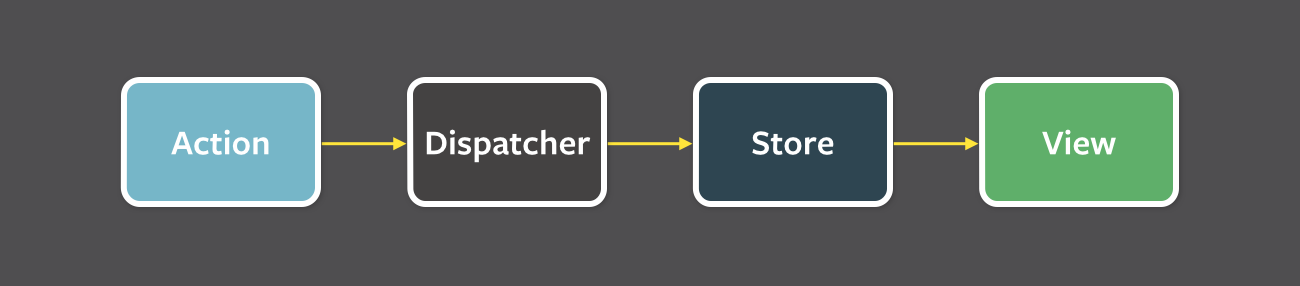
\includegraphics[scale=0.3]{img/Unidirectional.png}
\caption{Unidirectional Dataflow}
\end{figure}

\noindent Die Engine ``pusht'' den Applikationszustand in das
View-Layer, welches aus diesem ein User Interface rendert.
Die Interaktionen des Benutzers mit dem View-Layer erzeugen dann
wiederum Events, die als Streams an die Engine zurückfließen, wo sie
interpretiert und verarbeitet werden. Das Interpretieren der Events
lässt sich, dank des deklarativen Stils den PureScript erlaubt, leicht
programmieren. Als Beispiel soll der Code dienen, der das Ziehen eines
Themas auf das Grid beschreibt.

\begin{lstlisting}
  dragTopic = do
    Right t <- dragStart
    action <- dragOver
    lookup "dragEndTopic" `merge` lookup "dragEndGridTopic"
    return $ action t
\end{lstlisting}
\noindent Hier werden die Eventstreams für den Beginn eines
Drag Vorgangs sowie das Ziehen über einen Zeitslot mit dem Beenden des
Drag Vorgangs kombiniert und in einem resultierenden Stream \texttt{dragTopic}
ausgegeben. Dieser Stream abstrahiert nun die Mechanik des Drag and
Drop Vorganges und erlaubt es die tatsächlichen Intentionen des
Nutzers zu modellieren,um angemessen auf diese reagieren zu können.
\subsection{Test \& Abnahme}
Der Client wurde auf verschiedenen Endgeräten getestet. Hierbei fielen
immer wieder Kleinigkeiten auf, die sich unterschieden. Das fixen
dieser kleinen Bugs gestaltete sich als zu zeitaufwendig, und so wurden
die unterstützten Browser auf Firefox und Chrome festgelegt.
Die Mobile Version wurde sowohl auf Android als auch auf iOS ausgiebig
getestet und funktioniert ohne Einschränkungen auf beiden Systemen.
\subsection{Projektablauf}

%%% Local Variables:
%%% mode: latex
%%% TeX-master: "../Doku"
%%% End:
